\documentclass[11pt]{article}
%Gummi|065|=)

\usepackage{array}
\usepackage{graphicx}
\usepackage{tgschola}
\usepackage{algorithmic}
\usepackage{amssymb}
\usepackage{amsmath}
\DeclareMathOperator*{\argmax}{argmax}

\title{\textbf{SSU : Assignment 5} \\ \textbf{Windy world, Reinforcement learning}}
\author{\textbf{Teymur Azayev}}
\date{}


\begin{document}

\maketitle

\section{Overview}
This document is a short report for the fifth assignment from the subject. It includes a theoretical overview of the task, an explanation of the implementation, results and a short discussion.

\section{Task}
The task is to find an optimal policy function in the windy griworld environment. The task
is posed as a standard reinforcement learning problem for the MDP defined by the gridworld environment.
We will take a look at using a few different algorithms for finding the optimal policy, both directly and indirectly. 


\section{Value iteration}
We will first use a value iteration approach to finding the optimal Q-function (action value function). 
The algorithm converges in 683 epochs to the optimal Q-value, meaning the Q-matrix for which we get the maximal reward out of our MDP, in this case -15. We use a maximum of 100 iterations per epoch. Below is the Q matrix for each of the actions in order and the policy plotted in the gridworld.

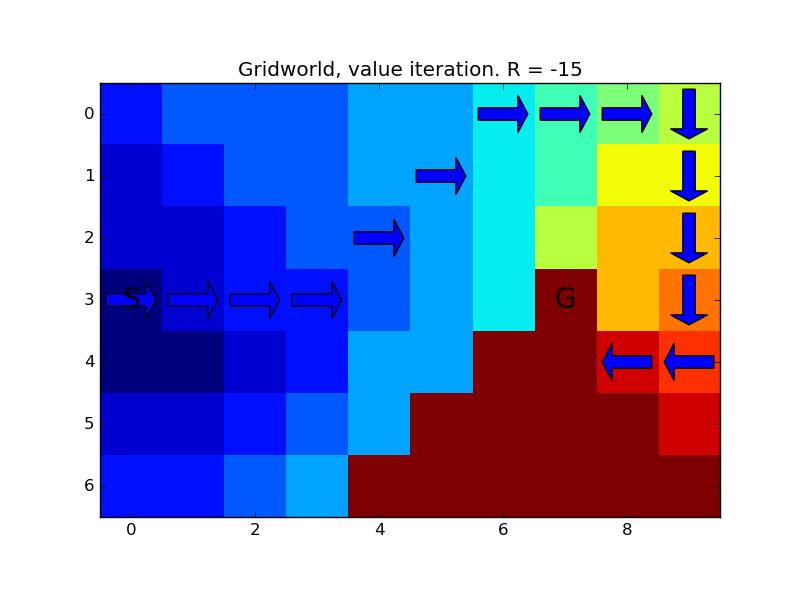
\includegraphics[width=11cm]{actionvaluepolicy.png}
\\
Action: Left
\[
\begin{bmatrix}
  -13. & -13. & -12. & -11. & -11. & -10. & -10. & -9. & -8. & -7.\\
  -14. & -13. & -12. & -12. & -11. & -11. & -10. & -9. & -9. & -6.\\
  -14. & -14. & -13. & -12. & -12. & -11. & -10. & -6. & -9. & -5.\\
  -15. & -14. & -13. & -13. & -12. & -12. & -10. & 0. & -7. & -5.\\
  -15. & -15. & -14. & -13. & -12. & -11. & 0. & -8. & -1. & -2.\\
  -14. & -14. & -13. & -12. & -10. & 0. & 0. & -7. & -1. & -1.\\
  -13. & -13. & -13. & -12. & 0. & 0. & 0. & 0. & -1. & -1.\\
\end{bmatrix} 
\]
Action: Right
\[
\begin{bmatrix}
  -12. & -12. & -11. & -11. & -10. & -10. & -9. & -8. & -7. & -7.\\
  -13. & -12. & -11. & -11. & -10. & -10. & -9. & -8. & -5. & -6.\\
  -14. & -13. & -12. & -11. & -11. & -10. & -9. & -6. & -5. & -5.\\
  -14. & -13. & -12. & -12. & -11. & -10. & -9. & 0. & -5. & -4.\\
  -15. & -14. & -13. & -12. & -11. & -10. & 0. & 0. & -3. & -2.\\
  -14. & -13. & -12. & -11. & -10. & 0. & 0. & 0. & 0. & -1.\\
  -12. & -12. & -11. & -10. & 0. & 0. & 0. & 0. & 0. & 0.\\
\end{bmatrix}
\]
Action: Up
\[
\begin{bmatrix}
  -12. & -11. & -12. & -11. & -11. & -11. & -9. & -9. & -7. & -7.\\
  -13. & -12. & -11. & -11. & -10. & -10. & -9. & -9. & -7. & -6.\\
  -14. & -13. & -12. & -11. & -11. & -10. & -10. & -8. & -5. & -6.\\
  -14. & -14. & -13. & -12. & -11. & -11. & -9. & 0. & -5. & -4.\\
  -15. & -14. & -13. & -12. & -12. & -11. & 0. & 0. & -5. & -2.\\
  -14. & -14. & -12. & -12. & -11. & 0. & 0. & 0. & 0. & -2.\\
  -12. & -12. & -12. & -11. & 0. & 0. & 0. & 0. & 0. & 0.\\
\end{bmatrix}
\]
Action: Down
\[
\begin{bmatrix}
  -12. & -12. & -11. & -12. & -10. & -10. & -10. & -8. & -8. & -6.\\
  -14. & -14. & -13. & -12. & -10. & -10. & -9. & -8. & -6. & -5.\\
  -13. & -13. & -12. & -12. & -12. & -10. & -10. & -6. & -4. & -4.\\
  -15. & -13. & -12. & -12. & -12. & -10. & -10. & 0. & -4. & -3.\\
  -14. & -14. & -13. & -12. & -10. & -10. & 0. & 0. & -2. & -2.\\
  -13. & -13. & -12. & -12. & -10. & 0. & 0. & 0. & 0. & -1.\\
  -12. & -12. & -12. & -10. & 0. & 0. & 0. & 0. & 0. & 0.\\
\end{bmatrix}
\]

\section{SARSA}
For the SARSA algorithm we use a greedy policy with eploration noise coefficients $\epsilon$ in ranges of $\{ 0.01, 0.1, 0.3\}$ and learning rates $\alpha$ of $\{ 0.01, 0.1, 0.3\}$ . Below are the plots for each algorithm. We can see that an $\epsilon$ of $0.01$ gives the most stable results, with higher epsilon giving divergent behavior for higher learning rates. We can also note that a learning rate of $0.01$ is too little and take too long to converge.

\begin{figure}[htp]

\centering
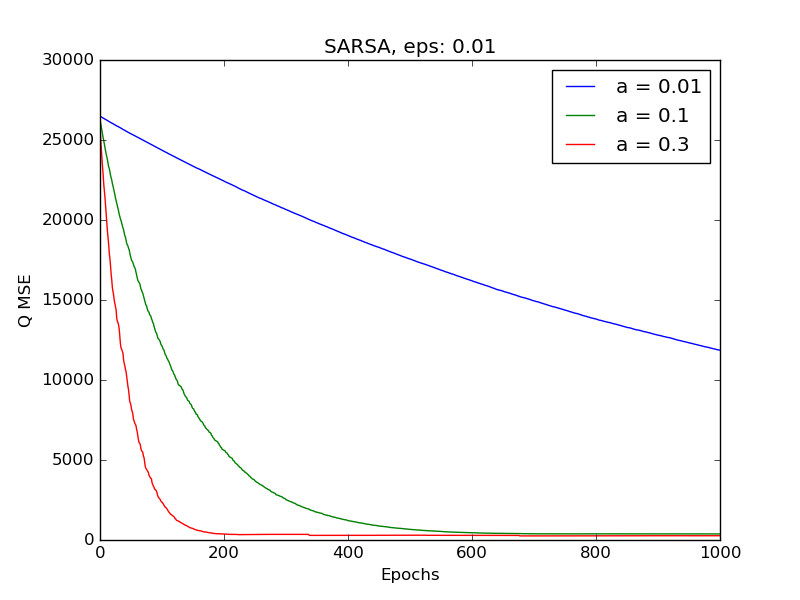
\includegraphics[width=.33\textwidth]{sarsaeps001}\hfill
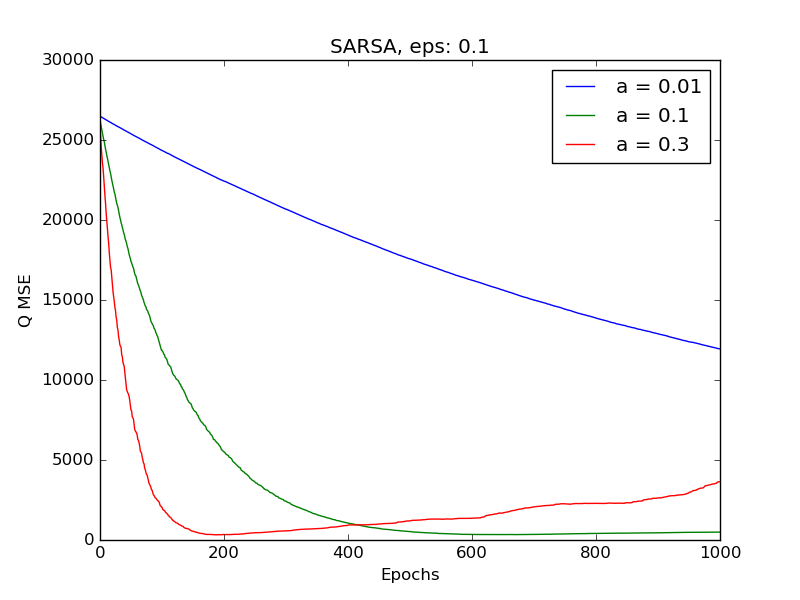
\includegraphics[width=.33\textwidth]{sarsaeps01}\hfill
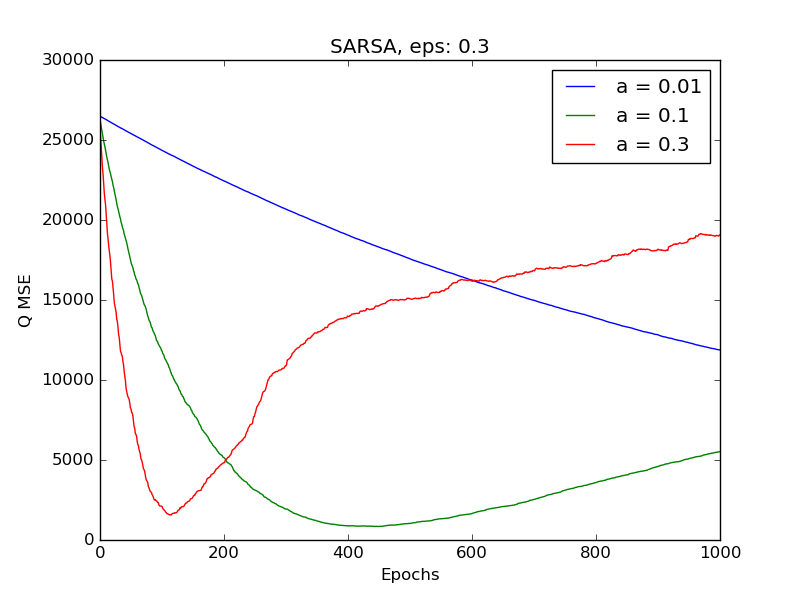
\includegraphics[width=.33\textwidth]{sarsaeps03}

\caption{default}
\label{fig:figure3}

\end{figure}

\section{Q-learning}
For the Q-learning (SARSA-max) algorithm we also use a greedy policy with eploration noise coefficients $\epsilon$ in ranges of $\{ 0.01, 0.1, 0.3\}$ and learning rates $\alpha$ of $\{ 0.01, 0.1, 0.3\}$ . Below are the plots for each algorithm. We can see that an $\epsilon$ of $0.01$ gives the most stable results, with higher epsilon giving divergent behavior for higher learning rates.

\begin{figure}[htp]

\centering
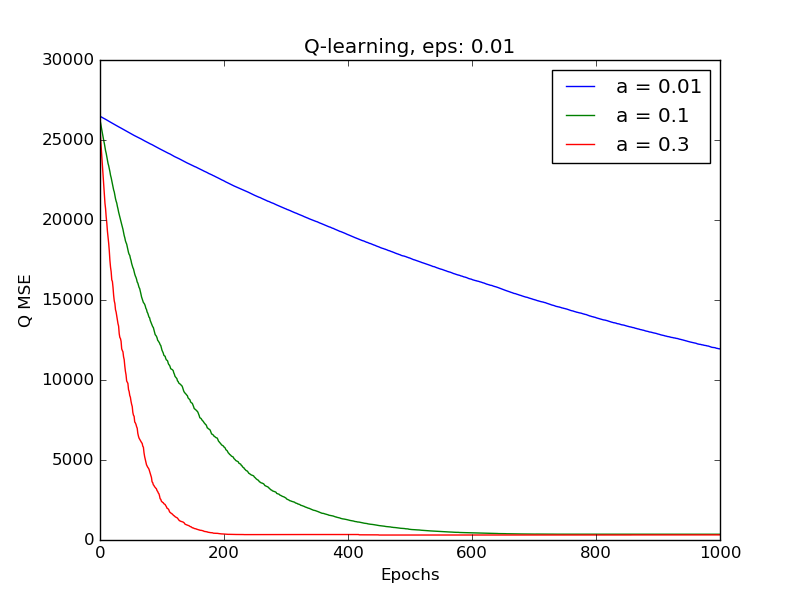
\includegraphics[width=.33\textwidth]{qleps001}\hfill
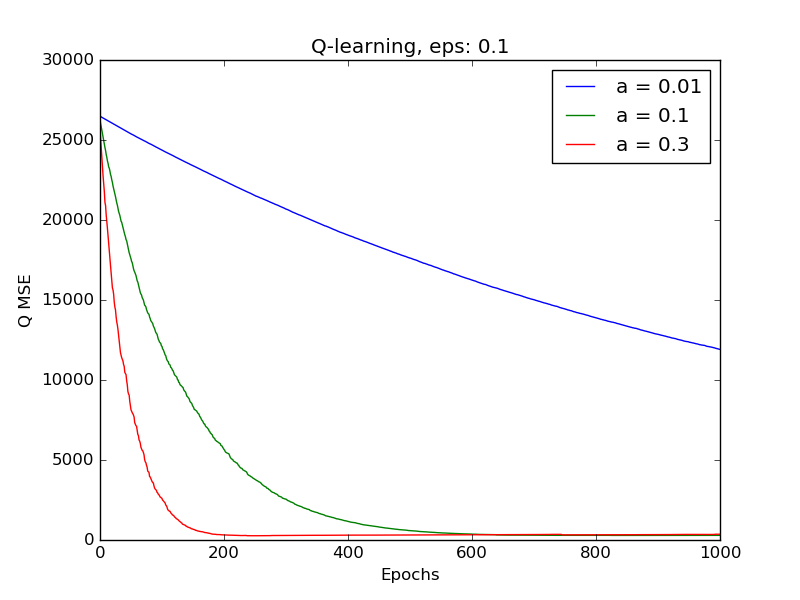
\includegraphics[width=.33\textwidth]{qleps01}\hfill
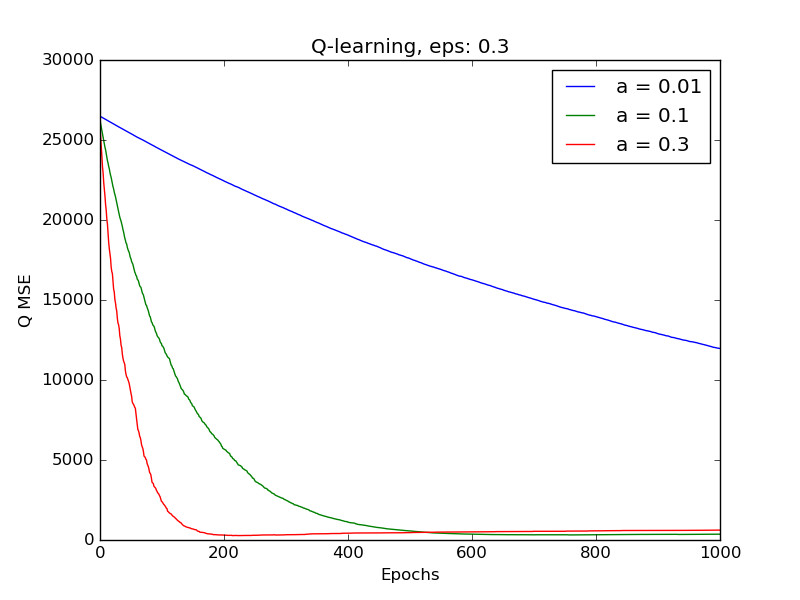
\includegraphics[width=.33\textwidth]{qleps03}

\caption{default}
\label{fig:figure3}

\end{figure}

\section{Discussion}


\section{Conclusion}
This concludes the report on this task.


\end{document}
